% ╔══════════════════════════════════════════════════════════════════════════╗
% ║  CS 173 — TikZ Diagrams & Math Guide                                    ║
% ║  Compile with pdflatex.  This file IS the guide — read the source.      ║
% ╚══════════════════════════════════════════════════════════════════════════╝

\documentclass[11pt]{article}
\usepackage[margin=1in]{geometry}
\usepackage{amsmath, amssymb, amsthm}
\usepackage{mathtools}
\usepackage{xcolor}
\usepackage{mdframed}
\usepackage{enumitem}
\usepackage{hyperref}
\usepackage{pagecolor}
\usepackage{microtype}
\usepackage{listings}           % for showing LaTeX source inline
\usepackage{multicol}           % two-column reference tables

% ── TikZ and all libraries used in this guide ─────────────────────────────────
\usepackage{tikz}
\usetikzlibrary{
  arrows.meta,
  positioning,
  shapes.geometric,
  calc,
  patterns,
  decorations.pathreplacing,
  fit,
  backgrounds,
  matrix,
}

% ── Colours ───────────────────────────────────────────────────────────────────
\definecolor{cream}{HTML}{FFFDF5}
\definecolor{defblue}{HTML}{1A4A7A}
\definecolor{thmgreen}{HTML}{1A5C3A}
\definecolor{warnAmber}{HTML}{7A4A00}
\definecolor{boxbluebg}{HTML}{EBF3FB}
\definecolor{boxgreenbg}{HTML}{EBF7EF}
\definecolor{boxamberbg}{HTML}{FDF5E6}
\pagecolor{cream}

% ── lstlistings style for showing code ────────────────────────────────────────
\lstset{
  language=[LaTeX]TeX,
  basicstyle=\ttfamily\small,
  backgroundcolor=\color{boxbluebg},
  frame=single, framerule=0.4pt,
  breaklines=true,
  columns=flexible,
  keywordstyle=\color{defblue},
  commentstyle=\color{gray},
}

% ── Shorthands ────────────────────────────────────────────────────────────────
\newcommand{\N}{\mathbb{N}}
\newcommand{\Z}{\mathbb{Z}}
\newcommand{\R}{\mathbb{R}}
\newcommand{\Pow}{\mathcal{P}}
\newcommand{\abs}[1]{\lvert #1 \rvert}
\newcommand{\setst}[2]{\{#1 \mid #2\}}

% ── Theorem environments ──────────────────────────────────────────────────────
\newmdenv[backgroundcolor=boxbluebg, linecolor=defblue, linewidth=2pt,
  topline=false, rightline=false, bottomline=false,
  innerleftmargin=10pt, innerrightmargin=10pt,
  innertopmargin=6pt, innerbottommargin=6pt, skipabove=8pt, skipbelow=8pt]{defbox}

\newmdenv[backgroundcolor=boxgreenbg, linecolor=thmgreen, linewidth=2pt,
  topline=false, rightline=false, bottomline=false,
  innerleftmargin=10pt, innerrightmargin=10pt,
  innertopmargin=6pt, innerbottommargin=6pt, skipabove=8pt, skipbelow=8pt]{thmbox}

\newmdenv[backgroundcolor=boxamberbg, linecolor=warnAmber, linewidth=2pt,
  topline=false, rightline=false, bottomline=false,
  innerleftmargin=10pt, innerrightmargin=10pt,
  innertopmargin=6pt, innerbottommargin=6pt, skipabove=8pt, skipbelow=8pt]{notebox}

% ── Section colours ───────────────────────────────────────────────────────────
\usepackage{titlesec}
\titleformat{\section}{\large\bfseries\color{defblue}}{}{0pt}{}[\titlerule]
\titleformat{\subsection}{\normalsize\bfseries\color{thmgreen}}{}{0pt}{}

% ──────────────────────────────────────────────────────────────────────────────
\begin{document}

\begin{center}
  {\Large\bfseries CS 173 --- Diagrams \& Math Reference Guide}\\[4pt]
  {\normalsize TikZ, proof typesetting, and CS173 notation}\\[2pt]
  {\small\color{gray} University of Illinois at Urbana-Champaign}
\end{center}
\vspace{0.5em}\hrule\vspace{1.5em}

\tableofcontents
\newpage

% ══════════════════════════════════════════════════════════════════════════════
\section{Graph Theory Diagrams}
% ══════════════════════════════════════════════════════════════════════════════

\subsection{Simple undirected graph}

%  Nodes at named positions, edges drawn between them.
\begin{center}
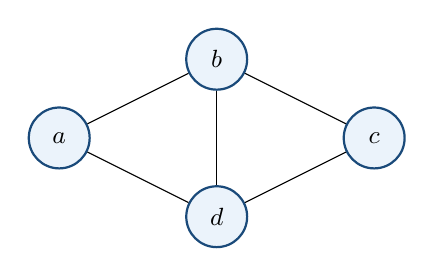
\begin{tikzpicture}[
    vertex/.style={circle, draw=defblue, fill=boxbluebg, thick,
                   minimum size=22pt, font=\small\bfseries},
    every edge/.style={draw=defblue, thick},
  ]
  \node[vertex] (a) at (0,0)   {$a$};
  \node[vertex] (b) at (2,1)   {$b$};
  \node[vertex] (c) at (4,0)   {$c$};
  \node[vertex] (d) at (2,-1)  {$d$};

  \draw (a) -- (b) -- (c) -- (d) -- (a);
  \draw (b) -- (d);
\end{tikzpicture}
\end{center}

\begin{lstlisting}
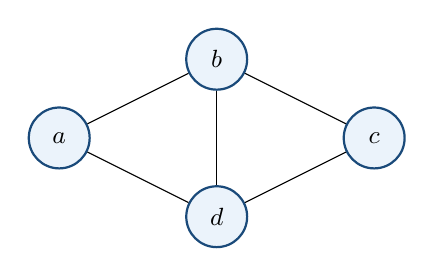
\begin{tikzpicture}[
    vertex/.style={circle, draw=defblue, fill=boxbluebg, thick,
                   minimum size=22pt, font=\small\bfseries},
  ]
  \node[vertex] (a) at (0,0)  {$a$};
  \node[vertex] (b) at (2,1)  {$b$};
  \node[vertex] (c) at (4,0)  {$c$};
  \node[vertex] (d) at (2,-1) {$d$};

  \draw (a) -- (b) -- (c) -- (d) -- (a);
  \draw (b) -- (d);
\end{tikzpicture}
\end{lstlisting}

\subsection{Directed graph (digraph)}

\begin{center}
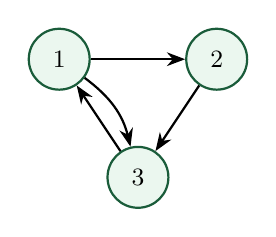
\begin{tikzpicture}[
    vertex/.style={circle, draw=thmgreen, fill=boxgreenbg, thick,
                   minimum size=22pt, font=\small\bfseries},
    ->, >=Stealth, thick,
  ]
  \node[vertex] (1) at (0,0)  {$1$};
  \node[vertex] (2) at (2,0)  {$2$};
  \node[vertex] (3) at (1,-1.5) {$3$};

  \draw (1) -- (2);
  \draw (2) -- (3);
  \draw (3) -- (1);
  \draw (1) edge[bend left=20] (3);
\end{tikzpicture}
\end{center}

\begin{lstlisting}
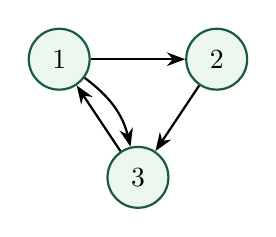
\begin{tikzpicture}[
    vertex/.style={circle, draw=thmgreen, fill=boxgreenbg, thick,
                   minimum size=22pt},
    ->, >=Stealth, thick,
  ]
  \node[vertex] (1) at (0,0)    {$1$};
  \node[vertex] (2) at (2,0)    {$2$};
  \node[vertex] (3) at (1,-1.5) {$3$};

  \draw (1) -- (2);
  \draw (2) -- (3);
  \draw (3) -- (1);
  \draw (1) edge[bend left=20] (3);   % curved arrow
\end{tikzpicture}
\end{lstlisting}

\subsection{Bipartite graph}

\begin{center}
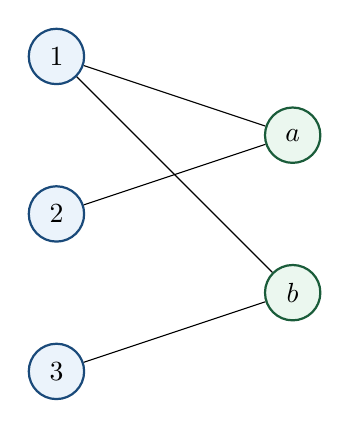
\begin{tikzpicture}[
    L/.style={circle, draw=defblue,  fill=boxbluebg,  thick, minimum size=20pt},
    R/.style={circle, draw=thmgreen, fill=boxgreenbg, thick, minimum size=20pt},
    every edge/.style={draw=gray!70, thick},
  ]
  \foreach \i/\y in {1/2, 2/0, 3/-2}
    \node[L] (l\i) at (0,\y) {$\i$};

  \foreach \i/\y in {a/1, b/-1}
    \node[R] (r\i) at (3,\y) {$\i$};

  \draw (l1)--(ra); \draw (l1)--(rb);
  \draw (l2)--(ra);
  \draw (l3)--(rb);
\end{tikzpicture}
\end{center}

\begin{lstlisting}
% Two node styles for the two parts
\node[L] (l1) at (0, 2) {$1$};  \node[L] (l2) at (0, 0) {$2$};
\node[R] (ra) at (3, 1) {$a$};  \node[R] (rb) at (3,-1) {$b$};
\draw (l1)--(ra); \draw (l1)--(rb); \draw (l2)--(ra);
\end{lstlisting}

\subsection{Edge labels}

\begin{center}
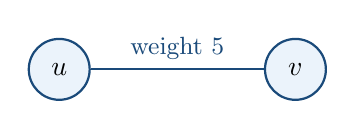
\begin{tikzpicture}[vertex/.style={circle, draw=defblue, fill=boxbluebg,
    thick, minimum size=22pt}]
  \node[vertex] (u) at (0,0) {$u$};
  \node[vertex] (v) at (3,0) {$v$};
  \draw[thick, defblue] (u) -- node[above, font=\small]{weight $5$} (v);
\end{tikzpicture}
\end{center}

\begin{lstlisting}
\draw (u) -- node[above, font=\small]{weight $5$} (v);
\end{lstlisting}

\subsection{Self-loops}

\begin{lstlisting}
\draw (v) edge[loop above] node{} (v);
\end{lstlisting}

% ══════════════════════════════════════════════════════════════════════════════
\section{Set Diagrams (Venn Diagrams)}
% ══════════════════════════════════════════════════════════════════════════════

\subsection{Two-set Venn diagram}

\begin{center}
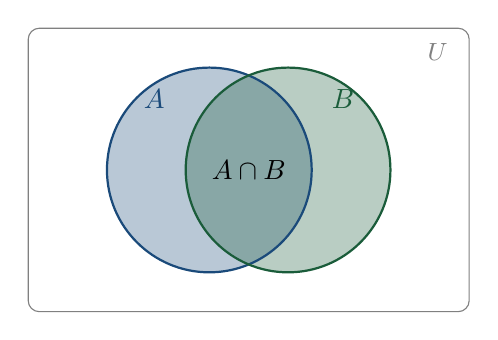
\begin{tikzpicture}
  \def\radius{1.3}
  \def\overlap{1.0}
  % filled regions
  \begin{scope}[fill opacity=0.3]
    \fill[defblue] (-\overlap/2, 0) circle (\radius);
    \fill[thmgreen] ( \overlap/2, 0) circle (\radius);
  \end{scope}
  % outlines
  \draw[defblue,  thick] (-\overlap/2, 0) circle (\radius);
  \draw[thmgreen, thick] ( \overlap/2, 0) circle (\radius);
  % labels
  \node at (-\overlap/2 - 0.7, 0.9) {\color{defblue}$A$};
  \node at ( \overlap/2 + 0.7, 0.9) {\color{thmgreen}$B$};
  \node at (0, 0) {$A \cap B$};
  % universe box
  \draw[gray, rounded corners] (-2.8,-1.8) rectangle (2.8,1.8);
  \node[gray, font=\small] at (2.4, 1.5) {$U$};
\end{tikzpicture}
\end{center}

\begin{lstlisting}
\def\radius{1.3} \def\overlap{1.0}
\begin{scope}[fill opacity=0.3]
  \fill[defblue]  (-\overlap/2, 0) circle (\radius);
  \fill[thmgreen] ( \overlap/2, 0) circle (\radius);
\end{scope}
\draw[defblue,  thick] (-\overlap/2, 0) circle (\radius);
\draw[thmgreen, thick] ( \overlap/2, 0) circle (\radius);
\node at (-\overlap/2 - 0.7, 0.9) {\color{defblue}$A$};
\node at ( \overlap/2 + 0.7, 0.9) {\color{thmgreen}$B$};
\end{lstlisting}

\subsection{Subset diagram ($A \subseteq B$)}

\begin{center}
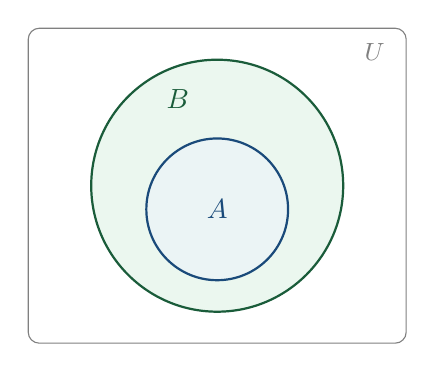
\begin{tikzpicture}
  \draw[thmgreen, thick, fill=boxgreenbg] (0,0) circle (1.6);
  \draw[defblue,  thick, fill=boxbluebg, fill opacity=0.5] (0,-0.3) circle (0.9);
  \node at (0,-0.3)  {\color{defblue}$A$};
  \node at (-0.5,1.1) {\color{thmgreen}$B$};
  \draw[gray, rounded corners] (-2.4,-2.0) rectangle (2.4,2.0);
  \node[gray, font=\small] at (2.0, 1.7) {$U$};
\end{tikzpicture}
\end{center}

\begin{lstlisting}
% Outer circle = B, inner circle = A
\draw[thmgreen, thick, fill=boxgreenbg] (0,0) circle (1.6);
\draw[defblue,  thick, fill=boxbluebg, fill opacity=0.5] (0,-0.3) circle (0.9);
\node at (0,-0.3)  {\color{defblue}$A$};
\node at (-0.5,1.1) {\color{thmgreen}$B$};
\end{lstlisting}

% ══════════════════════════════════════════════════════════════════════════════
\section{Function Diagrams}
% ══════════════════════════════════════════════════════════════════════════════

\subsection{Arrow diagram (mapping between finite sets)}

\begin{center}
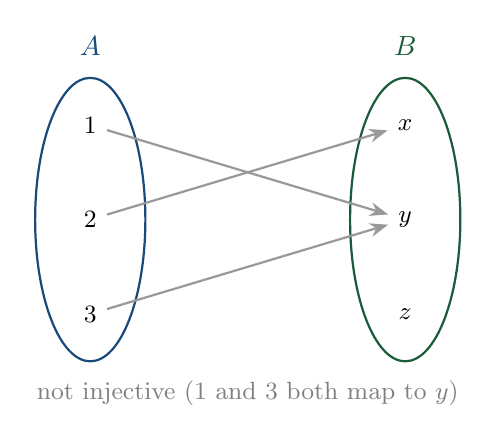
\begin{tikzpicture}[
    elem/.style={font=\small},
    ->, >=Stealth, thick,
  ]
  % Domain ellipse
  \draw[defblue, thick] (0,0) ellipse (0.7 and 1.8);
  \node[defblue, font=\bfseries] at (0, 2.2) {$A$};
  \node[elem] (a1) at (0, 1.2)  {$1$};
  \node[elem] (a2) at (0, 0)    {$2$};
  \node[elem] (a3) at (0,-1.2)  {$3$};

  % Codomain ellipse
  \draw[thmgreen, thick] (4,0) ellipse (0.7 and 1.8);
  \node[thmgreen, font=\bfseries] at (4, 2.2) {$B$};
  \node[elem] (b1) at (4, 1.2)  {$x$};
  \node[elem] (b2) at (4, 0)    {$y$};
  \node[elem] (b3) at (4,-1.2)  {$z$};

  % Mapping arrows
  \draw[gray!80] (a1) -- (b2);
  \draw[gray!80] (a2) -- (b1);
  \draw[gray!80] (a3) -- (b2);

  \node[font=\small, gray] at (2, -2.2) {not injective (1 and 3 both map to $y$)};
\end{tikzpicture}
\end{center}

\begin{lstlisting}
% Draw domain ellipse
\draw[defblue, thick] (0,0) ellipse (0.7 and 1.8);
\node (a1) at (0, 1.2) {$1$};  \node (a2) at (0,0) {$2$};

% Draw codomain ellipse
\draw[thmgreen, thick] (4,0) ellipse (0.7 and 1.8);
\node (b1) at (4, 1.2) {$x$};  \node (b2) at (4,0) {$y$};

% Arrows
\draw[->, >=Stealth, gray!80] (a1) -- (b2);
\draw[->, >=Stealth, gray!80] (a2) -- (b1);
\end{lstlisting}

\subsection{Bijection diagram}

\begin{center}
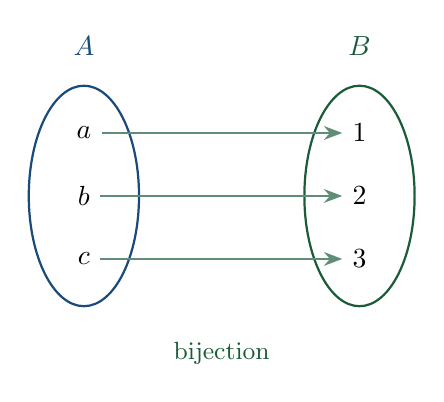
\begin{tikzpicture}[->, >=Stealth, thick]
  \draw[defblue, thick] (0,0) ellipse (0.7 and 1.4);
  \node[defblue, font=\bfseries] at (0, 1.9) {$A$};
  \node (a1) at (0, 0.8)  {$a$};
  \node (a2) at (0, 0)    {$b$};
  \node (a3) at (0,-0.8)  {$c$};

  \draw[thmgreen, thick] (3.5,0) ellipse (0.7 and 1.4);
  \node[thmgreen, font=\bfseries] at (3.5, 1.9) {$B$};
  \node (b1) at (3.5, 0.8)  {$1$};
  \node (b2) at (3.5, 0)    {$2$};
  \node (b3) at (3.5,-0.8)  {$3$};

  \draw[thmgreen!70] (a1) -- (b1);
  \draw[thmgreen!70] (a2) -- (b2);
  \draw[thmgreen!70] (a3) -- (b3);
  \node[font=\small, thmgreen] at (1.75, -2.0) {bijection};
\end{tikzpicture}
\end{center}

% ══════════════════════════════════════════════════════════════════════════════
\section{Hasse Diagrams (Partial Orders)}
% ══════════════════════════════════════════════════════════════════════════════

Hasse diagrams omit arrows (direction is up) and transitive edges.

\begin{center}
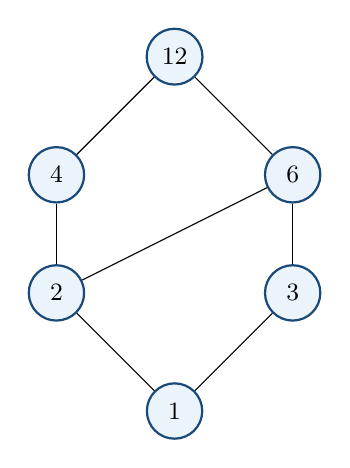
\begin{tikzpicture}[
    node/.style={circle, draw=defblue, fill=boxbluebg, thick,
                 minimum size=20pt, font=\small},
    every edge/.style={draw=defblue!70, thick},
  ]
  % Divisibility on {1,2,3,4,6,12}
  \node[node] (1)  at (0,0)   {$1$};
  \node[node] (2)  at (-1.5,1.5) {$2$};
  \node[node] (3)  at (1.5,1.5)  {$3$};
  \node[node] (4)  at (-1.5,3)   {$4$};
  \node[node] (6)  at (1.5,3)    {$6$};
  \node[node] (12) at (0,4.5)    {$12$};

  \draw (1)--(2); \draw (1)--(3);
  \draw (2)--(4); \draw (2)--(6); \draw (3)--(6);
  \draw (4)--(12); \draw (6)--(12);
\end{tikzpicture}
\end{center}

\begin{lstlisting}
% Divisibility poset on {1,2,3,4,6,12} — only cover relations drawn
\node[node] (1)  at (0,0)      {$1$};
\node[node] (2)  at (-1.5,1.5) {$2$};   \node[node] (3) at (1.5,1.5) {$3$};
\node[node] (4)  at (-1.5,3)   {$4$};   \node[node] (6) at (1.5,3)   {$6$};
\node[node] (12) at (0,4.5)    {$12$};
\draw (1)--(2); \draw (1)--(3); \draw (2)--(4); \draw (2)--(6);
\draw (3)--(6); \draw (4)--(12); \draw (6)--(12);
\end{lstlisting}

% ══════════════════════════════════════════════════════════════════════════════
\section{Trees (Induction / Graph Theory)}
% ══════════════════════════════════════════════════════════════════════════════

\subsection{Binary tree}

\begin{center}
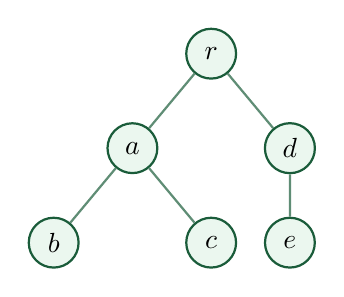
\begin{tikzpicture}[
    n/.style={circle, draw=thmgreen, fill=boxgreenbg, thick, minimum size=18pt},
    level distance=1.2cm,
    sibling distance=2.0cm,
    edge from parent/.style={draw=thmgreen!70, thick},
  ]
  \node[n] {$r$}
    child { node[n] {$a$}
      child { node[n] {$b$} }
      child { node[n] {$c$} }
    }
    child { node[n] {$d$}
      child { node[n] {$e$} }
    };
\end{tikzpicture}
\end{center}

\begin{lstlisting}
\usepackage{tikz}   % child/sibling syntax is built in

\begin{tikzpicture}[level distance=1.2cm, sibling distance=2.0cm]
  \node[n] {$r$}
    child { node[n] {$a$}
      child { node[n] {$b$} }
      child { node[n] {$c$} }
    }
    child { node[n] {$d$}
      child { node[n] {$e$} }
    };
\end{tikzpicture}
\end{lstlisting}

\subsection{Labelling leaf nodes differently}

\begin{lstlisting}
% Define two node styles
\tikzstyle{inner} = [circle, draw=thmgreen, fill=boxgreenbg, thick, minimum size=18pt]
\tikzstyle{leaf}  = [circle, draw=warnAmber, fill=boxamberbg, thick, minimum size=18pt]

\node[inner] {$r$}
  child { node[inner] {$v$}
    child { node[leaf] {$\ell_1$} }
    child { node[leaf] {$\ell_2$} }
  };
\end{lstlisting}

% ══════════════════════════════════════════════════════════════════════════════
\section{Induction Proof Structure}
% ══════════════════════════════════════════════════════════════════════════════

\begin{notebox}
Use the \texttt{description} environment for the standard three-part layout.
\end{notebox}

\begin{lstlisting}
\begin{proof}[Proof by (strong) induction on $n$]
  \begin{description}[leftmargin=2cm, labelwidth=2cm]

    \item[Base case.] ($n = 0$) ...

    \item[IH.] Assume $P(k)$ holds for all $k < n$.

    \item[IS.] We show $P(n)$ ...

  \end{description}
\end{proof}
\end{lstlisting}

Rendered output:

\begin{thmbox}
\begin{proof}[Proof by strong induction on $n$]
  \begin{description}[leftmargin=2cm, labelwidth=2cm]
    \item[Base case.] ($n = 0$)\quad $P(0)$ holds because \ldots
    \item[IH.] Assume $P(k)$ holds for all $0 \le k < n$.
    \item[IS.] We show $P(n)$\ldots \qedhere
  \end{description}
\end{proof}
\end{thmbox}

% ══════════════════════════════════════════════════════════════════════════════
\section{Aligned Proof Steps with Justifications}
% ══════════════════════════════════════════════════════════════════════════════

Use \texttt{align} or \texttt{alignat} to line up equals signs and add reasons.

\begin{lstlisting}
\begin{align*}
  |A \cup B| &= |A| + |B| - |A \cap B|  & \text{(inclusion-exclusion)}  \\
             &= 5 + 7 - 3                & \text{(given)}                \\
             &= 9.
\end{align*}
\end{lstlisting}

\begin{thmbox}
\begin{align*}
  |A \cup B| &= |A| + |B| - |A \cap B|  & \text{(inclusion-exclusion)}  \\
             &= 5 + 7 - 3                & \text{(given)}                \\
             &= 9.
\end{align*}
\end{thmbox}

\subsection{Cases}

\begin{lstlisting}
\begin{proof}
  We consider two cases.
  \begin{description}
    \item[Case 1: $n$ even.] Write $n = 2k$. Then \ldots
    \item[Case 2: $n$ odd.]  Write $n = 2k+1$. Then \ldots
  \end{description}
\end{proof}
\end{lstlisting}

% ══════════════════════════════════════════════════════════════════════════════
\section{Truth Tables}
% ══════════════════════════════════════════════════════════════════════════════

\begin{center}
\begin{tabular}{c c | c | c | c}
  $P$ & $Q$ & $P \land Q$ & $P \lor Q$ & $P \Rightarrow Q$ \\
  \hline
  T & T & T & T & T \\
  T & F & F & T & F \\
  F & T & F & T & T \\
  F & F & F & F & T \\
\end{tabular}
\end{center}

\begin{lstlisting}
\begin{tabular}{c c | c | c | c}
  $P$ & $Q$ & $P \land Q$ & $P \lor Q$ & $P \Rightarrow Q$ \\
  \hline
  T & T & T & T & T \\
  T & F & F & T & F \\
  F & T & F & T & T \\
  F & F & F & F & T \\
\end{tabular}
\end{lstlisting}

% ══════════════════════════════════════════════════════════════════════════════
\section{Counting / Combinatorics}
% ══════════════════════════════════════════════════════════════════════════════

\begin{multicols}{2}
\subsection*{Binomial coefficients}
\begin{lstlisting}
\binom{n}{k}     % C(n,k)
\end{lstlisting}

\subsection*{Permutations / products}
\begin{lstlisting}
\prod_{i=1}^{n} a_i
\sum_{k=0}^{n} \binom{n}{k}
\end{lstlisting}
\end{multicols}

\subsection{Pigeonhole illustration}

\begin{center}
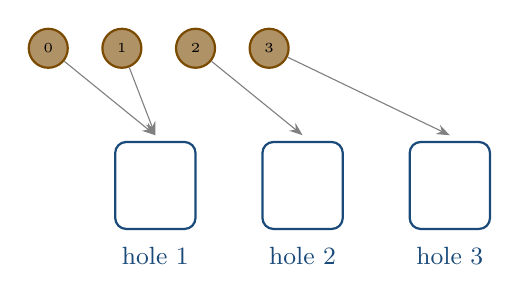
\begin{tikzpicture}[scale=0.85]
  % 3 holes
  \foreach \i in {1,2,3} {
    \draw[defblue, thick, rounded corners=4pt]
      ({(\i-1)*2.2 - 0.6}, -0.5) rectangle ({(\i-1)*2.2 + 0.6}, 0.8);
    \node[defblue, font=\small] at ({(\i-1)*2.2}, -0.9) {hole $\i$};
  }
  % 4 pigeons (circles above, arrows down)
  \foreach \j/\hole in {0/1, 1/1, 2/2, 3/3} {
    \node[circle, fill=warnAmber!60, draw=warnAmber, thick,
          minimum size=14pt, font=\tiny] (p\j)
      at ({(\j)*1.1 - 1.6}, 2.2) {$\j$};
  }
  \draw[->, >=Stealth, gray] (p0) -- (0,0.9);
  \draw[->, >=Stealth, gray] (p1) -- (0,0.9);
  \draw[->, >=Stealth, gray] (p2) -- (2.2,0.9);
  \draw[->, >=Stealth, gray] (p3) -- (4.4,0.9);
\end{tikzpicture}
\end{center}

% ══════════════════════════════════════════════════════════════════════════════
\section{Cardinality \& Cantor Diagrams}
% ══════════════════════════════════════════════════════════════════════════════

\subsection{Diagonal argument schematic}

\begin{center}
\begin{tikzpicture}[font=\ttfamily\small]
  \node at (-1.5, 0) {$f(1) =$};
  \node at (-1.5,-0.8) {$f(2) =$};
  \node at (-1.5,-1.6) {$f(3) =$};
  \node at (-1.5,-2.4) {\vdots};

  \foreach \i/\row in {
    1/{0,1,1,0,\ldots},
    2/{1,0,0,1,\ldots},
    3/{0,0,1,1,\ldots}}{
    \node at (0.8, {(1-\i)*0.8}) {$\row$};
  }

  % Highlight diagonal
  \draw[dangerRed, very thick]
    (0,  0.15) rectangle (0.32,-0.15);
  \draw[dangerRed, very thick]
    (0.65,-0.65) rectangle (0.97,-0.95);
  \draw[dangerRed, very thick]
    (1.35,-1.45) rectangle (1.67,-1.75);

  \node[dangerRed, font=\small\bfseries] at (0.8, -3.0)
    {flip diagonal $\Rightarrow$ new sequence not in list};
\end{tikzpicture}
\end{center}

% ══════════════════════════════════════════════════════════════════════════════
\section{CS 173 Math Symbol Quick Reference}
% ══════════════════════════════════════════════════════════════════════════════

\begin{center}
\begin{tabular}{l l l}
  \textbf{Meaning} & \textbf{Command} & \textbf{Output} \\
  \hline
  Natural numbers     & \texttt{\textbackslash{}mathbb\{N\}} & $\mathbb{N}$ \\
  Integers            & \texttt{\textbackslash{}mathbb\{Z\}} & $\mathbb{Z}$ \\
  Reals               & \texttt{\textbackslash{}mathbb\{R\}} & $\mathbb{R}$ \\
  Power set           & \texttt{\textbackslash{}mathcal\{P\}(A)} & $\mathcal{P}(A)$ \\
  Set-builder         & \texttt{\textbackslash\{x \textbackslash{}mid P(x)\textbackslash\}} & $\{x \mid P(x)\}$ \\
  Cardinality         & \texttt{\textbackslash{}lvert A \textbackslash{}rvert} & $\lvert A \rvert$ \\
  Divides             & \texttt{a \textbackslash{}mid b} & $a \mid b$ \\
  Does not divide     & \texttt{a \textbackslash{}nmid b} & $a \nmid b$ \\
  Modulo              & \texttt{a \textbackslash{}equiv b \textbackslash{}pmod\{n\}} & $a \equiv b \pmod{n}$ \\
  For all             & \texttt{\textbackslash{}forall} & $\forall$ \\
  There exists        & \texttt{\textbackslash{}exists} & $\exists$ \\
  Implies             & \texttt{\textbackslash{}Rightarrow} & $\Rightarrow$ \\
  Iff                 & \texttt{\textbackslash{}iff} & $\iff$ \\
  Negation            & \texttt{\textbackslash{}lnot} & $\lnot$ \\
  Conjunction         & \texttt{\textbackslash{}land} & $\land$ \\
  Disjunction         & \texttt{\textbackslash{}lor} & $\lor$ \\
  Subset              & \texttt{\textbackslash{}subseteq} & $\subseteq$ \\
  Proper subset       & \texttt{\textbackslash{}subsetneq} & $\subsetneq$ \\
  Intersection        & \texttt{\textbackslash{}cap} & $\cap$ \\
  Union               & \texttt{\textbackslash{}cup} & $\cup$ \\
  Set difference      & \texttt{A \textbackslash{}setminus B} & $A \setminus B$ \\
  Empty set           & \texttt{\textbackslash{}emptyset} & $\emptyset$ \\
  Contradiction       & \texttt{\textbackslash{}Rightarrow\textbackslash{}Leftarrow} & $\Rightarrow\Leftarrow$ \\
  Floor               & \texttt{\textbackslash{}lfloor x \textbackslash{}rfloor} & $\lfloor x \rfloor$ \\
  Ceiling             & \texttt{\textbackslash{}lceil x \textbackslash{}rceil} & $\lceil x \rceil$ \\
  Composition         & \texttt{f \textbackslash{}circ g} & $f \circ g$ \\
  \hline
\end{tabular}
\end{center}

% ══════════════════════════════════════════════════════════════════════════════
\section{Useful TikZ Tips}
% ══════════════════════════════════════════════════════════════════════════════

\begin{defbox}
\textbf{Relative node placement} — use \texttt{positioning} library:
\begin{lstlisting}
\usetikzlibrary{positioning}
\node (a) {$a$};
\node[right=1.5cm of a] (b) {$b$};   % 1.5cm to the right of a
\node[below=of b]       (c) {$c$};   % default gap below b
\end{lstlisting}
\end{defbox}

\begin{defbox}
\textbf{Foreach loops} — draw grids, regular polygons, etc.:
\begin{lstlisting}
\foreach \i in {0,60,...,300} {
  \node[circle, fill=defblue!30] at (\i:1.5) {};
}
\end{lstlisting}
\end{defbox}

\begin{defbox}
\textbf{Curly brace annotation} — label a span of nodes:
\begin{lstlisting}
\usetikzlibrary{decorations.pathreplacing}
\draw[decorate, decoration={brace, amplitude=6pt}]
  (0,0) -- (3,0) node[midway, below=8pt]{$n$ elements};
\end{lstlisting}
\end{defbox}

\begin{defbox}
\textbf{Wrapping TikZ in a figure}:
\begin{lstlisting}
\begin{figure}[h]
  \centering
  \begin{tikzpicture} ... \end{tikzpicture}
  \caption{A graph on 4 vertices.}
  \label{fig:mygraph}
\end{figure}
% Reference with \ref{fig:mygraph}
\end{lstlisting}
\end{defbox}

\end{document}
